\documentclass[tikz,border=2pt]{standalone}
\usepackage{amsmath}
\usetikzlibrary{arrows.meta}
\newcommand{\angl}[1]{\overline{#1|}}
\begin{document}
% Two-year temporary life annuities with v = 0.95, 1p_x = 0.9, 2p_x = 0.8: the due version pays at 0 and 1
% (APV 1 + 0.95(0.9) = 1.855), the immediate version at 1 and 2 (APV 0.95(0.9) + 0.95^2(0.8) = 1.577);
% each payment at time k contributes v^k kp_x, and later whole-life payments (grey) are cut off.
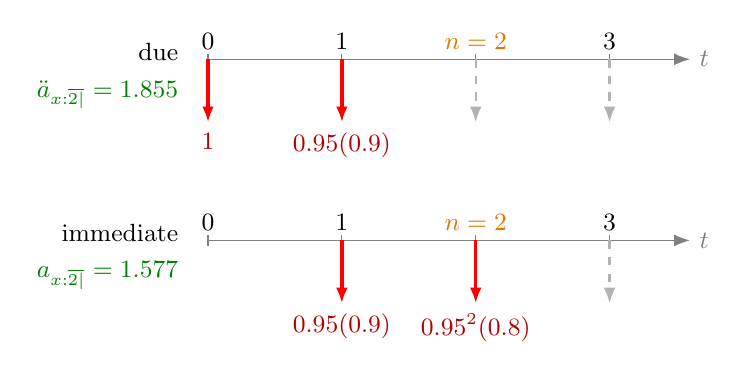
\begin{tikzpicture}[font=\small, >={Latex[length=2mm]}, x=1.7cm]
  \newcommand{\taxis}{%
    \draw[gray, ->] (0,0) -- (3.6,0) node[right] {$t$};
    \foreach \t in {0,1,3} {\draw[gray] (\t,-0.07) -- (\t,0.07); \node[above, inner sep=2pt] at (\t,0.05) {$\t$};}
    \draw[gray] (2,-0.07) -- (2,0.07);
    \node[orange!90!black, above, inner sep=2pt] at (2,0.05) {$n=2$};}
  % annuity-due
  \taxis
  \node[anchor=east] at (-0.15,0.1) {due};
  \node[green!50!black, anchor=east] at (-0.15,-0.45) {$\ddot a_{x:\angl{2}}=1.855$};
  \draw[red, very thick, ->] (0,0) -- (0,-0.8) node[below, red!70!black] {$1$};
  \draw[red, very thick, ->] (1,0) -- (1,-0.8) node[below, red!70!black] {$0.95(0.9)$};
  \foreach \t in {2,3} \draw[gray!60, thick, dashed, ->] (\t,0) -- (\t,-0.8);
  % annuity-immediate
  \begin{scope}[yshift=-2.3cm]
    \taxis
    \node[anchor=east] at (-0.15,0.1) {immediate};
    \node[green!50!black, anchor=east] at (-0.15,-0.45) {$a_{x:\angl{2}}=1.577$};
    \draw[red, very thick, ->] (1,0) -- (1,-0.8) node[below, red!70!black] {$0.95(0.9)$};
    \draw[red, very thick, ->] (2,0) -- (2,-0.8) node[below, red!70!black] {$0.95^2(0.8)$};
    \draw[gray!60, thick, dashed, ->] (3,0) -- (3,-0.8);
  \end{scope}
\end{tikzpicture}
\end{document}
